% 编译：在本文件所在目录运行 XeLaTeX 两遍。
% 完整源码直接读取同目录 ThreeFourOne.lean，避免另存一份代码后发生不同步。
\documentclass[UTF8,fontset=fandol,a4paper,11pt]{ctexart}
\usepackage[margin=25mm]{geometry}
\usepackage{amsmath,amssymb,mathtools}
\usepackage{xcolor}
\usepackage{graphicx,caption}
\usepackage{fontspec}
\setmonofont{DejaVuSansMono.ttf}[BoldFont=DejaVuSansMono-Bold.ttf,Scale=0.88]
\usepackage{fancyvrb,fvextra}
\usepackage{booktabs,array,enumitem,needspace,fancyhdr,xurl,hyperref}
\hypersetup{colorlinks=true,linkcolor=blue!45!black,urlcolor=blue!45!black,
  pdftitle={ThreeFourOne.lean 逐步说明：3–4–1 三角不等式}}
\fvset{fontsize=\small,breaklines=true,breakanywhere=false,
  frame=leftline,framesep=5pt,xleftmargin=8pt}
\setlength{\emergencystretch}{2em}
\setlength{\parskip}{0.3em}
\linespread{1.15}
\setlist{itemsep=0.15em,topsep=0.3em}
\pagestyle{fancy}
\fancyhf{}
\fancyhead[L]{\small 形式化证明：逐步阅读}
\fancyhead[R]{\small 3–4–1 三角不等式}
\fancyfoot[C]{\thepage}
\setlength{\headheight}{15pt}
\newcommand{\code}[1]{{\small\ttfamily\def\_{\textunderscore\allowbreak}#1}}
\pdfstringdefDisableCommands{\def\code#1{#1}}
\newcommand{\step}[1]{\Needspace{7\baselineskip}\subsection{#1}}
\title{\texttt{ThreeFourOne.lean} 逐步说明\\[0.3em]\large 从倍角公式到 3–4–1 三角不等式}
\author{}
\date{2026 年 10 月 28 日草案}

\begin{document}
\maketitle

本文对同目录的 \code{ThreeFourOne.lean} 作逐步说明。目标不是系统讲授 Lean，
而是通过一个完整的小证明，说明数学推理如何写成可由计算机核验的形式。
阅读时只需熟悉余弦倍角公式、实数平方非负及通常的代数运算。
全文区分三件事：要证明的数学命题、代码如何组织推理，以及编辑器当前显示的信息。

\section{先看数学证明}

对任意实数 $\theta$，要证明
\begin{equation}\label{eq:target}
  3+4\cos\theta+\cos(2\theta)\ge0.
\end{equation}
其中三个余弦项的系数依次为 $3,4,1$，因而称为 3–4–1 三角不等式。
这是一个对所有实数成立的精确不等式，不是若干角度的数值检验。

证明由两个步骤组成。首先使用倍角公式
\[
  \cos(2\theta)=2\cos^2\theta-1,
\]
得到
\begin{align*}
  3+4\cos\theta+\cos(2\theta)
  &=3+4\cos\theta+2\cos^2\theta-1\\
  &=2+4\cos\theta+2\cos^2\theta\\
  &=2(1+\cos\theta)^2.
\end{align*}
其次，因为 $1+\cos\theta$ 是实数，故
\[
  (1+\cos\theta)^2\ge0.
\]
再乘以非负实数 $2$，即得式~\eqref{eq:target}。

代码也分成这两个命题：先证明恒等式，再由恒等式推出非负性。
这样第二个证明能明确调用第一个证明，而不必重新展开倍角公式。

\clearpage
\section{完整代码与阅读约定}

下面直接读取同目录的实际源码；左边的数字是源码行号，不属于 Lean 程序。
\VerbatimInput[fontsize=\footnotesize,numbers=left,numbersep=5pt]{ThreeFourOne.lean}

\paragraph{怎样理解“每一步”}
代码中的空行用于分隔内容，注释用于解释意图，真正构成证明的是命题陈述和
\code{by} 后的指令。以下先解释文件准备部分，再逐条说明两个证明。
后文显示的目标为便于阅读作了排版整理，编辑器中的换行、隐含参数或类型标记可能略有差别。

\Needspace{9\baselineskip}
\section{文件准备：导入、注释与名字空间}

\step{导入三角函数的基础理论}
\begin{Verbatim}
import Mathlib.Analysis.SpecialFunctions.Trigonometric.Basic
\end{Verbatim}
\code{import} 表示载入一个模块及其依赖。这里导入的是 mathlib 中三角函数的基础理论，
包括实余弦函数 \code{Real.cos} 和本例使用的倍角公式 \code{Real.cos\_two\_mul}。

这一步没有证明本例的目标，也没有调用已经完成的 3–4–1 不等式。
它提供的是推理所需的基础对象与一般结果，类似于通常数学证明引用已知的倍角公式。

\step{导入证明策略}
\begin{Verbatim}
import Mathlib.Tactic
\end{Verbatim}
这一行载入 mathlib 的证明策略，其中本例实际使用了 \code{ring} 和 \code{norm\_num}。
前者处理多项式恒等变形，后者处理数值命题。
导入策略不表示由某个外部计算器宣布结论正确：策略产生的证明仍须交给 Lean 内核检查。

\step{识别两种注释}
\begin{Verbatim}
/-!
这里是跨越多行的说明文字。
-/

-- 这里是只到本行末尾的注释。
\end{Verbatim}
\code{/-!} 与 \code{-/} 之间是模块文档注释；\code{--} 之后到本行末尾是单行注释。
其中的中文帮助人理解代码，但不参与命题的证明。
Lean 接受代码并不意味着它也核验了中文注释与数学原意的一致性；这一点仍须人工检查。

\step{把定理放入名字空间}
\begin{Verbatim}
namespace Progressive
\end{Verbatim}
\code{namespace} 用于组织名称，避免与其他文件中的同名定理混淆。
在这一范围内写出的 \code{three\_four\_one\_identity}，其完整名称是
\code{Progressive.three\_four\_one\_identity}。
文件末尾的
\begin{Verbatim}
end Progressive
\end{Verbatim}
只表示结束这个名字空间，不是额外的数学推理。

\section{第一个定理：证明恒等式}

\step{逐项读出定理陈述}
\begin{Verbatim}
theorem three_four_one_identity (θ : ℝ) :
    3 + 4 * Real.cos θ + Real.cos (2 * θ)
      = 2 * (1 + Real.cos θ) ^ 2 := by
\end{Verbatim}
这里为适应说明文档的行宽，将原陈述换行显示；数学内容与源码一致。

\begin{description}[style=nextline,leftmargin=1.5em]
  \item[\code{theorem}]
  声明一个有证明的定理。其后必须提供能通过检查的证明，不能只写出定理名称。
  \item[\code{three\_four\_one\_identity}]
  是定理名称，供后文引用。名称本身不参与推理。
  \item[\code{(θ : ℝ)}]
  声明参数 $\theta$ 是实数。冒号在这里表示“具有类型”。因为未对 $\theta$ 加其他条件，
  定理对每个实数 $\theta$ 都成立；其逻辑内容相当于“对所有 $\theta\in\mathbb R$”。
  \item[参数之后的冒号]
  引出要证明的命题，即下一行的等式。
  \item[\code{Real.cos θ}]
  表示实余弦函数作用于实数 $\theta$，相当于通常写法 $\cos\theta$。
  Lean 用空格表示函数应用，不要求写成 \code{Real.cos(θ)}。
  \item[\code{*}、\code{+} 与 \code{\textasciicircum}]
  分别表示乘法、加法和乘方。因此 \code{(1 + Real.cos θ) \textasciicircum\ 2}
  是 $1+\cos\theta$ 的平方，不是只对余弦项平方。
  \item[\code{:= by}]
  \code{:=} 引出所提供的证明，\code{by} 表示使用策略式证明。
  这里不是重新定义余弦，也不是先假定这个等式成立。
\end{description}

在 \code{by} 后、尚未执行任何策略时，证明状态可读作
\begin{Verbatim}
θ : ℝ
⊢ 3 + 4 * Real.cos θ + Real.cos (2 * θ)
    = 2 * (1 + Real.cos θ) ^ 2
\end{Verbatim}
横线或符号 \code{⊢} 上方列出当前可用的参数与事实，下方是尚须证明的目标。
这里仅有参数 $\theta$，还没有额外的假设。

\step{第一条指令：用倍角公式改写目标}
\begin{Verbatim}
rw [Real.cos_two_mul]
\end{Verbatim}
\code{rw} 是改写策略。方括号中给出要使用的等式；在本行没有加反向标记，
所以按该等式从左到右改写。
\code{Real.cos\_two\_mul} 的数学内容是
\[
  \cos(2\theta)=2\cos^2\theta-1.
\]
Lean 从当前目标中的 \code{Real.cos (2 * θ)} 自动识别出参数 $\theta$，
因此无须另写“将倍角公式中的变量取为 $\theta$”。

执行后，目标成为
\begin{Verbatim}
θ : ℝ
⊢ 3 + 4 * Real.cos θ + (2 * Real.cos θ ^ 2 - 1)
    = 2 * (1 + Real.cos θ) ^ 2
\end{Verbatim}
注意，目标此时并未完成：倍角项消除了，但两边仍须作代数比较。
\code{rw} 改变的是待证表达式的形式，不是把一个尚未证明的命题当作事实加入。

\step{第二条指令：核验多项式恒等式}
\begin{Verbatim}
ring
\end{Verbatim}
此时把 $c=\cos\theta$ 看成一个实数量，目标就是
\[
  3+4c+(2c^2-1)=2(1+c)^2.
\]
\code{ring} 将两边按照环的运算规则化为可比较的标准形式，核对常数项、一次项和二次项。
其内容相当于
\[
  3+4c+2c^2-1=2c^2+4c+2
  =2(1+2c+c^2).
\]
它不需要知道 $c$ 是余弦值，也不使用 $-1\le\cos\theta\le1$。
换言之，三角函数的知识已经在上一条倍角公式中使用，剩余部分是纯代数恒等变形。

核验完成后，不再剩余待证目标。第一个定理因此成立，
可以在第二个定理中以它的名称作为已证明结果引用。

\section{第二个定理：推出非负性}

\step{读出第二个目标}
\begin{Verbatim}
theorem three_four_one_nonnegative (θ : ℝ) :
    0 ≤ 3 + 4 * Real.cos θ + Real.cos (2 * θ) := by
\end{Verbatim}
其结构与第一个定理相同。区别在于，这次目标是不等式而不是等式。
Lean 将“表达式大于等于零”写成“零小于等于表达式”，二者数学上完全相同。

初始状态为
\begin{Verbatim}
θ : ℝ
⊢ 0 ≤ 3 + 4 * Real.cos θ + Real.cos (2 * θ)
\end{Verbatim}

\step{第一条指令：调用自己刚证明的恒等式}
\begin{Verbatim}
rw [three_four_one_identity]
\end{Verbatim}
这里调用的不是 mathlib 中已经完成的目标不等式，而是本文件上一段实际证明的恒等式。
由于处于同一名字空间，可以省略名称前面的 \code{Progressive.}。

Lean 自动把恒等式中的参数匹配为当前的 $\theta$，将不等式右端改写为平方的两倍。
新目标是
\begin{Verbatim}
θ : ℝ
⊢ 0 ≤ 2 * (1 + Real.cos θ) ^ 2
\end{Verbatim}
本行承担数学证明中的承上启下：后续只需证明这个乘积非负，不必再处理倍角项。

\step{第二条指令：证明并命名一个中间事实}
\begin{Verbatim}
have hSquare : 0 ≤ (1 + Real.cos θ) ^ 2 := sq_nonneg _
\end{Verbatim}
这一行可以按四部分读出。
\begin{enumerate}
  \item \code{have}：提出一个即将被证明并加入当前上下文的中间事实。
  \item \code{hSquare}：为这一事实取名。它不是某个实数变量，而是一份给定命题的证明。
  \item 冒号后写出命题 $0\le(1+\cos\theta)^2$。
  \item \code{:=} 后提供证明 \code{sq\_nonneg \_}。
\end{enumerate}

一般引理 \code{sq\_nonneg} 的内容是：对任意实数 $a$，$a^2\ge0$。
下划线 \code{\_} 让 Lean 根据左边声明的命题推断应取的实数，
此处就是 $a=1+\cos\theta$。它不是漏掉证明，也不是跳过检查的占位符；
Lean 必须能够补出合适的表达式并检查其类型，才能接受这一行。

数学上，这一行就是
\[
  1+\cos\theta\in\mathbb R
  \quad\Longrightarrow\quad
  (1+\cos\theta)^2\ge0.
\]
不需要先证明 $1+\cos\theta\ge0$，因为实数平方无论底数正负都非负。

执行 \code{have} 之后，主目标没有消失，只是增加了可用事实：
\begin{Verbatim}
θ : ℝ
hSquare : 0 ≤ (1 + Real.cos θ) ^ 2
⊢ 0 ≤ 2 * (1 + Real.cos θ) ^ 2
\end{Verbatim}
这说明 \code{hSquare} 不是已经证明整个定理，而是证明了最后一步需要的一个组成部分。

\step{第三条指令：由两个非负因子完成证明}
\begin{Verbatim}
exact mul_nonneg (by norm_num) hSquare
\end{Verbatim}
先看一般引理 \code{mul\_nonneg}：
\[
  0\le a,\quad 0\le b
  \quad\Longrightarrow\quad 0\le ab.
\]
根据当前目标，Lean 推断
\[
  a=2,\qquad b=(1+\cos\theta)^2.
\]
因此它需要两份证明：$0\le2$ 的证明，以及
$0\le(1+\cos\theta)^2$ 的证明。

\paragraph{第一个输入：\code{(by norm\_num)}}
括号内是一段局部证明。其待证命题由 \code{mul\_nonneg} 与当前目标推断为
\[
  0\le(2:\mathbb R).
\]
\code{norm\_num} 核验这个数值不等式。它没有用数值近似计算 $\cos\theta$，
也没有抽取若干 $\theta$ 作实验；任意实参数 $\theta$ 在这里完全没有参与数值计算。

\paragraph{第二个输入：\code{hSquare}}
它就是上一行已经得到的平方非负证明。将它交给 \code{mul\_nonneg}，
便得到当前所需的乘积非负结论。

\paragraph{最前面的 \code{exact}}
\code{exact} 要求后面的表达式恰好是一份当前目标的证明。
本行提供的证明类型正是 $0\le2(1+\cos\theta)^2$，故可以结束当前证明。
如果因子、指数或不等号方向不匹配，Lean 不会仅因代码看起来相似就接受。

整行可用普通数学语言读成：
\begin{quote}
因为 $2\ge0$，且已证明 $(1+\cos\theta)^2\ge0$，所以二者乘积非负。
\end{quote}
结合此前的恒等式改写，最终得到原来的 3–4–1 不等式。

\section{证明状态的连续变化}

下面把第二个定理的状态变化集中排列，便于与 InfoView 对照。
\begin{enumerate}
  \item \textbf{开始时：}目标为 $0\le3+4\cos\theta+\cos2\theta$。
  \item \textbf{执行 \code{rw} 后：}目标变为 $0\le2(1+\cos\theta)^2$。
  \item \textbf{执行 \code{have} 后：}目标仍为同一个乘积非负，但可用事实中新增
    \code{hSquare}，即平方非负的证明。
  \item \textbf{执行 \code{exact} 后：}非负乘积引理的两个输入均已提供，目标完成。
\end{enumerate}
第一项恒等式的变化更短：原等式先由倍角公式改写，再由 \code{ring} 完成代数核验。
两段证明都具有清楚的中间状态，并非一条直接调用目标定理的指令。

\section{在 VS Code 中操作并判断证明是否通过}

\step{打开项目，而不是只打开一个代码文件}
以下以已经安装 Lean 4 扩展、并已取得本仓库依赖的 VS Code 为前提。
如果尚未安装，可先在扩展面板中查找 Lean 4 并完成安装；不要把安装扩展与本例证明本身混为一件事。
\begin{enumerate}
  \item 在 VS Code 的“文件”菜单中选择“打开文件夹”（macOS 的菜单也可能显示为“打开”）。
  \item 选择仓库中的 \code{形式化证明-Lean示例} 文件夹。
    项目根目录应有配置文件 \code{lakefile.toml}、\code{lean-toolchain}，以及 \code{LeanExamples} 目录，
    不要仅以最内层的 \code{Progressive} 目录作为项目根目录。
  \item 在左侧资源管理器中依次展开 \code{LeanExamples}、\code{Progressive}，
    打开 \code{ThreeFourOne.lean}，等待 Lean 服务处理文件。
  \item 如果右侧尚无 InfoView，按 macOS 的 \code{Cmd+Shift+P} 或
    Windows/Linux 的 \code{Ctrl+Shift+P} 打开命令面板，搜索 \code{Infoview}，
    选择 Lean 4 提供的切换或显示 InfoView 命令。
  \item 后续只需移动光标观察证明状态；修改文件后先保存，并等待检查完成。
    不需要按 Python 程序的运行按钮，也不需要为了看到证明状态添加打印语句。
\end{enumerate}
项目而非单文件的打开方式，可参看 Lean 社区的项目使用说明\footnote{\url{https://leanprover-community.github.io/install/project.html}。界面文字会随 VS Code 与 Lean 扩展版本略有变化，本文以所示实例说明。}。
首次加载可能需要准备依赖；如果出现找不到 \code{Mathlib} 的错误，应先检查项目环境，
不能据此认定三角不等式的证明有错。

\step{随着光标位置逐步观察目标}
先把光标放在第一个定理的 \code{by} 后，查看要证明的恒等式。
随后移至 \code{rw [Real.cos\_two\_mul]} 的行末，再移至 \code{ring} 的行末，
对照前文已经列出的目标变化。信息面板根据光标位置更新；在命令前、命令内和命令后，
看到的内容可能不同。

然后依次查看第二个定理的 \code{rw}、\code{have hSquare} 和最后的 \code{exact}。
将光标放在最后一行末尾，可观察该证明完成后的状态；将光标放在同一行的
\code{hSquare} 上，则还可能看到这个局部表达式应具有的类型。
这两种显示提供的信息不同，并不冲突。

\step{对照实际截图理解各个栏目}
图~\ref{fig:infoview-success} 是本例第二个定理完成后的实际 InfoView 截图。
它保留编辑器的原始显示，不是另行编造的证明输出。

\begin{figure}[htbp]
  \centering
  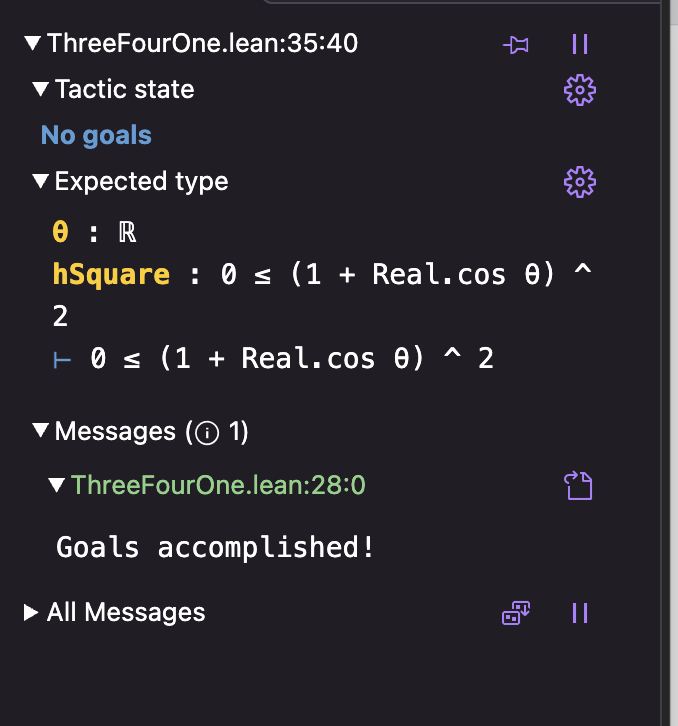
\includegraphics[width=0.58\textwidth,height=0.46\textheight,keepaspectratio]{ThreeFourOne-InfoView.png}
  \caption{第二个定理完成后的 InfoView。上方的 \texttt{No goals} 表示没有剩余目标；\texttt{Expected type} 显示所指局部证明的类型，并非新的未证目标。}
  \label{fig:infoview-success}
\end{figure}

各栏应分别理解：
\begin{enumerate}
  \item \code{ThreeFourOne.lean:35:40}：正在显示信息的文件和光标位置，
    后两项为行号、列号，不是错误编号。源码注释增减后，数字也会随之改变。
  \item \code{Tactic state} 下的 \code{No goals}：该位置的策略证明已经没有待处理目标。
    在本例最后一行，它表示非负性证明已经完成。
  \item \code{Expected type}：光标所指表达式在此处应当具有的类型。
    对证明表达式，类型就是命题；它不是报告错误的栏目。
  \item \code{θ : ℝ} 表明当前参数为实数；
    \code{hSquare : 0 ≤ (1 + Real.cos θ) \textasciicircum\ 2}
    表明已经具有平方非负的证明。符号 \code{⊢} 后再次出现同一命题，
    是因为最后一行的 \code{mul\_nonneg} 正需要这份证明作为第二个输入。
  \item \code{Messages} 中的 \code{Goals accomplished!}：编辑器针对相应定理的完成提示。
    图中的位置标记指向第二个定理的声明（本截图为第 28 行）。
    \code{Messages} 后的数字表示消息数量，不表示错误数量；消息的具体内容才决定其性质。
  \item \code{All Messages} 是可展开的消息列表。可在其中继续查看是否存在文件的其他错误，
    不能把这个栏目名称本身理解为通过或失败。
\end{enumerate}

图中 \code{Expected type} 内的平方指数 $2$ 因面板较窄而换行显示，
并非代码把平方写漏，也不是另外一条命题。
关键区别是：\code{Tactic state} 已没有未证目标，而 \code{Expected type}
仍可解释光标所指的一个证明对象为何适用于当前位置。

\step{什么情况下可以说“证明通过”}
在当前这个文件中，可以按以下层次作判断：
\begin{enumerate}
  \item 第一个定理末尾出现 \code{No goals}，表示恒等式的证明已完成。
  \item 第二个定理末尾出现 \code{No goals}，并有相应完成提示，表示非负性证明已完成。
  \item 保存文件并等待处理结束后，检查编辑器的问题面板及消息列表，没有本文件的错误；
    需要独立确认时，再执行下一节给出的命令行检查。
\end{enumerate}
这里的判断还依赖代码没有使用 \code{sorry} 等跳过证明的做法。
本例的两段证明均未使用此类占位，也未把目标命题声明为公理。
因此，本例的完成状态确实对应上述两条证明被 Lean 接受，而不只是证明框架暂时没有剩余目标。

单独一张 \code{No goals} 截图不能证明整个项目都正确，也不能检查中文解释是否忠实于数学原意。
它更不能表明本书后续的无零点论证已全部形式化。

\step{\code{No info found} 不是同一类提示}
\code{No info found} 表示编辑器在光标位置没有可显示的相应信息。
光标位于空行或注释时可能出现这一提示；它本身既不证明代码正确，也不说明代码错误。
可将光标移到 \code{rw}、\code{ring} 或 \code{exact} 等实际证明指令处查看状态。
如果仍无信息，再确认打开的是含 \code{lakefile.toml} 的项目文件夹，且 Lean 服务已完成加载。

\section{在本机核验与编译本文}

\step{使用项目环境核验 Lean 文件}
在 VS Code 中打开仓库下的 \code{形式化证明-Lean示例} 文件夹。
该文件夹包含 \code{lean-toolchain}、\code{lakefile.toml} 和本例使用的 mathlib 依赖。
在以这个文件夹为当前目录的终端中运行：
\begin{Verbatim}
lake env lean LeanExamples/Progressive/ThreeFourOne.lean
\end{Verbatim}
若终端当前位于 \code{Progressive} 子目录，应先回到项目根目录。
例如作者本机使用以下两行；其他读者将第一行替换为自己的项目路径：
\begin{Verbatim}
cd /Users/lichengtong/lichengtong-RH/形式化证明-Lean示例
lake env lean LeanExamples/Progressive/ThreeFourOne.lean
\end{Verbatim}
\code{lake env} 为随后启动的 Lean 设置项目环境，使其找到固定版本的依赖；
\code{lean} 检查后面指定的文件。这不是将文件编译成一个用于数值试验的程序，
而是检查其中的定义、命题和证明。

对于当前不含额外打印命令的 \code{ThreeFourOne.lean}，命令无错误退出时通常不会输出祝贺文字。
等到终端提示符重新出现，才表示这次命令已经结束；仍在运行时没有文字，不能提前判为成功。
如果只出现依赖库 \code{has local changes} 的警告，而命令正常退出，这不是证明错误，
但说明本次检查使用了存在本地改动的依赖目录，不能据此声称依赖与原始固定版本完全一致。
也可以运行 \code{lake build}，核验项目默认目标及其导入的模块。
这不等于机器上的所有任意 \code{.lean} 文件都已自动核验。

\step{查看定理的公理依赖}
在能找到该模块的项目环境中，可以另建临时审查文件，写入
\begin{Verbatim}
import LeanExamples.Progressive.ThreeFourOne

#print axioms Progressive.three_four_one_identity
#print axioms Progressive.three_four_one_nonnegative
\end{Verbatim}
先构建模块，再用 \code{lake env lean} 检查该临时文件。
本例当前核验得到的依赖为 Lean 的标准公理
\code{propext}、\code{Classical.choice}、\code{Quot.sound}，没有额外引入本例结论作公理，
也没有以 \code{sorry} 跳过证明。
这些标准公理属于所采用形式系统的基础；公理依赖检查不代替对命题含义及定义的人工核对。

\step{用 XeLaTeX 编译说明文档}
本文是独立的 TeX 文件，不需要导入全书。在本文与 \code{ThreeFourOne.lean} 所在目录执行两遍：
\begin{Verbatim}
xelatex -interaction=nonstopmode -halt-on-error ThreeFourOne-逐步说明.tex
\end{Verbatim}
本文、\code{ThreeFourOne.lean} 与截图 \code{ThreeFourOne-InfoView.png}
须放在同一目录，因为第二节通过 \code{\textbackslash VerbatimInput}
直接读取实际代码，截图也采用相对路径载入。中文字体采用 TeX Live 通常附带的 Fandol；
代码字体采用 DejaVu Sans Mono。若环境缺少该等宽字体，须先安装或替换为能显示
\code{θ}、\code{ℝ}、\code{≤} 等符号的等宽字体，不能忽略缺字警告。

\section{本例究竟核验了什么}

本例实际核验了以下推理链：
\[
  \text{倍角公式}
  \ \Longrightarrow\ 
  \text{恒等式}
  \ \Longrightarrow\ 
  \text{平方的两倍非负}
  \ \Longrightarrow\ 
  \text{3--4--1 不等式}.
\]
倍角公式、平方非负与乘积非负是引用的基础结果；代数整理、恒等式的组合及最后的非负性推导
是本例展开的内容。它没有重新建立实数理论或三角函数理论，也没有通过近似计算替代任意实参数下的证明。

本书随后将这一不等式用于构造关于 $\log|\zeta|$ 的非负组合。
从三角不等式到 $\zeta$ 的无零点结论，还需要级数展开、收敛性及极点附近的估计；
这些不属于 \code{ThreeFourOne.lean} 的证明范围，不能从本例通过检查直接推断后续结论已全部形式化。

\paragraph{阅读后的把握}
读者不必记住所有策略名称，但应能辨认每一步的输入与输出：
\code{rw} 用已经成立的等式改写目标，\code{have} 证明并保存中间事实，
\code{exact} 提交当前目标的证明；\code{ring} 与 \code{norm\_num}
分别完成限定范围内的代数与数值核验。这样便能理解一段短小的 Lean 证明为何成立，
以及它与通常数学证明究竟在哪些步骤上一一对应。

\end{document}
